\label{ch:supplementary_material}

\section*{Supplementary Material}
\beginsupplement

\begin{table}[!htbp]
	\centering
	\caption{List of the focal species observed in the natural condition experiment within the area of the Jena Experiment. Species had to flower in at least five plots with different frequency values.}
	\begin{tabular}{llllll}
		\toprule
		\textbf{Short} & \textbf{Name} & \textbf{German Name} & \textbf{Order} & \textbf{Family} & \textbf{Color} \\
		\midrule
		Ger   & \textit{Geranium pratense} & Wiesen-Storchschnabel & Geraniales & Geraniaceae & Purple \\
		Lat   & \textit{Lathyrus pratensis} & Wiesen-Platterbse & Fabales & Fabaceae & Yellow \\
		Lot   & \textit{Lathyrus pratensis} & Gewöhnliche Hornklee & Fabales & Fabaceae & Yellow \\
		Ono   & \textit{Onobrychis viciifolia} & Saat-Esparsette & Fabales & Fabaceae & pink+white \\
		TP    & \textit{Trifolium pratense} & Wiesen-Klee & Fabales & Fabaceae & Purple \\
		\bottomrule
	\end{tabular}%
	\label{tab:Species}
\end{table}%

%%%%%%%%%%%%%%%%%%%%%%%%%%

\begin{figure} [H] %plot-design
\centering
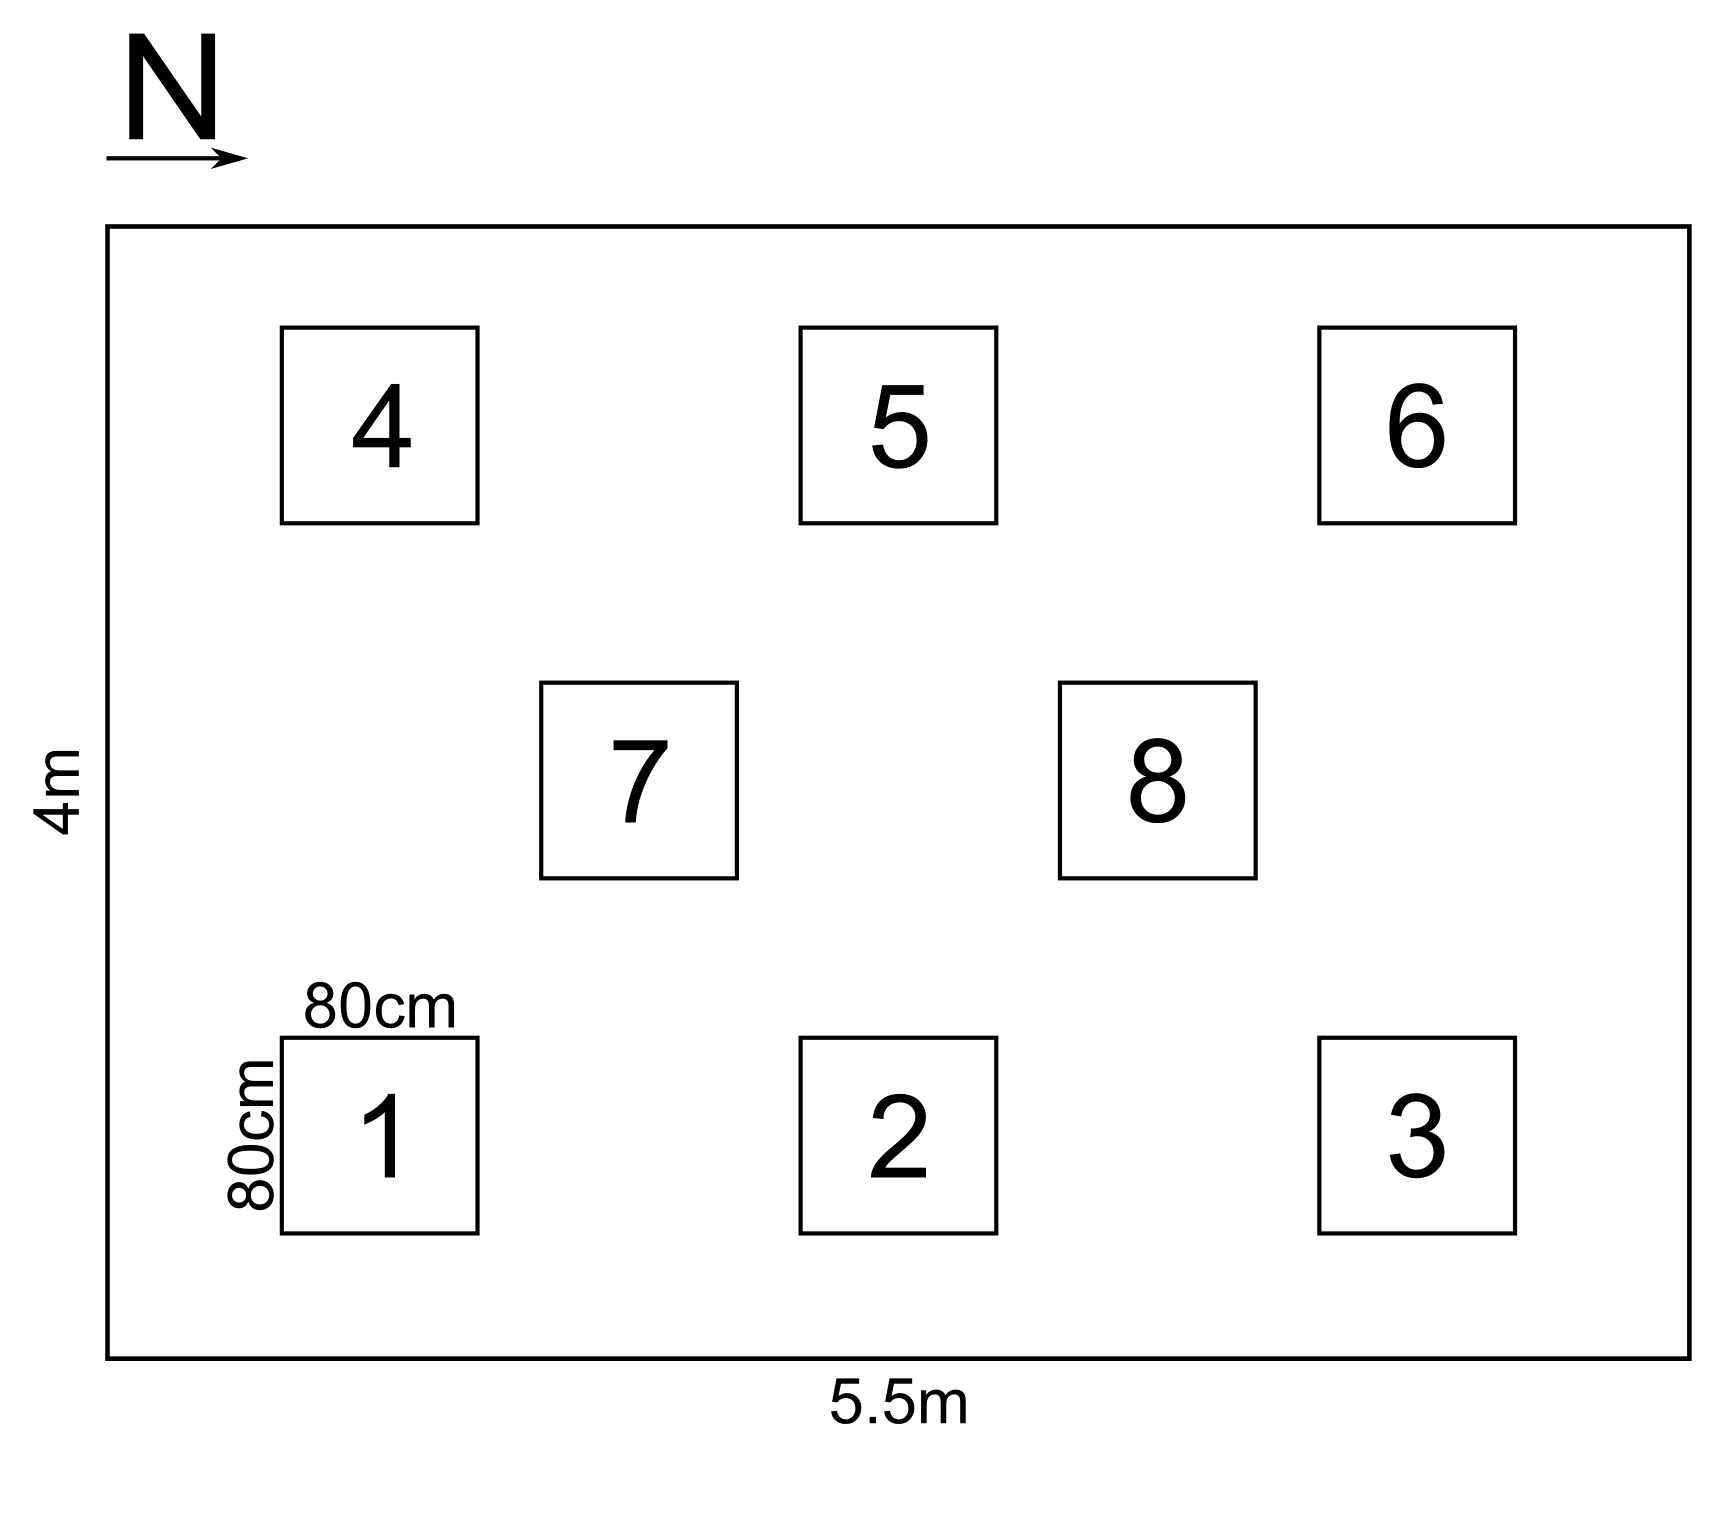
\includegraphics[width=9cm]{Images/plot-design}
 \caption{The distribution of subplots within the old invasion plots.}
 \label{fig:plot-design}
\end{figure}


%%%%%%%%%%%%%%%%%%%%%%%%%%
\newpage

\begin{figure} [H] %pairs-plot
\centering
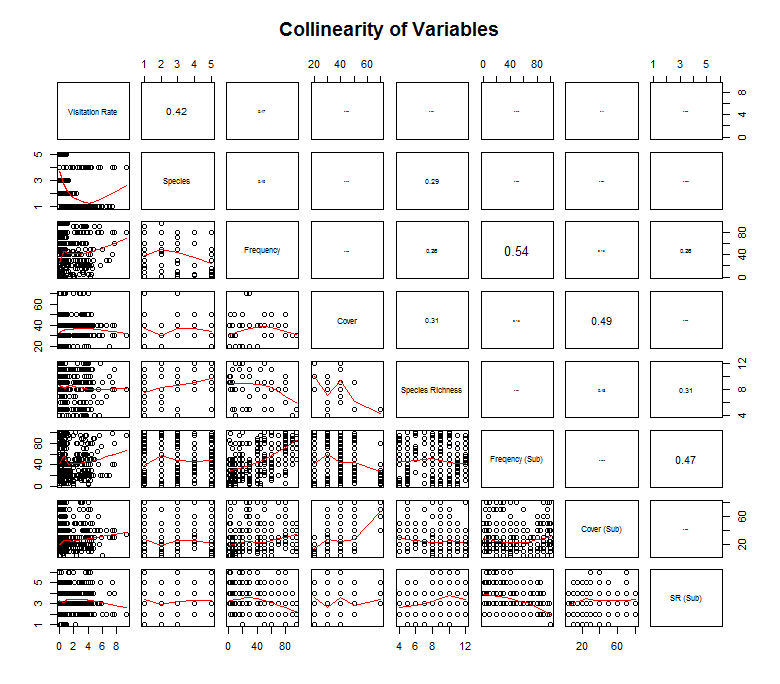
\includegraphics[width=16cm]{Images/pairs-plot}
 \caption{Pairwise correlation of Visitation rate (response variable), species, frequency, floral cover and species richness on plot and subplot-level. The upper panels contain Pearson correlation coefficients with its size proportional to its value. Parameters correlate on the plot and subplot level but show no strong correlation not among each other.}
 \label{fig:pairs-plot}
\end{figure}

%%%%%%%%%%%%%%%%%%%%%%%%%%

\begin{table}[!htbp] 
  \centering
  \caption{Variance inflation factors (VIF) for the full set of variables. Values are calculated by the "corvif"-function from R-package AED. All values are well below three indicating no collinearity (see \citet{zuur2007analysing}).}
  %cite for AED/Zuur
    \begin{tabular}{ll}
    \toprule
    \textbf{Variable} & \textbf{GVIF}\\
    \midrule
    Visitation Rate  	&  1.26\\
    Species 			 &  1.36\\
    Frequency 	  	    &  1.63\\
    Floral Cover   		 &  1.46\\
    Species Richness     &  1.45\\
    Frequency (Subplot) 	    &  1.84\\
    Floral Cover (Subplot)		  &  1.37\\
    Species Richness (Subplot)    &  1.48\\
    \bottomrule
    \end{tabular}%
\label{tab:VIF}
\end{table}%

%%%%%%%%%%%%%%%%%%%%%%%%%%
\clearpage

\begin{figure} [H] %residuals
\centering
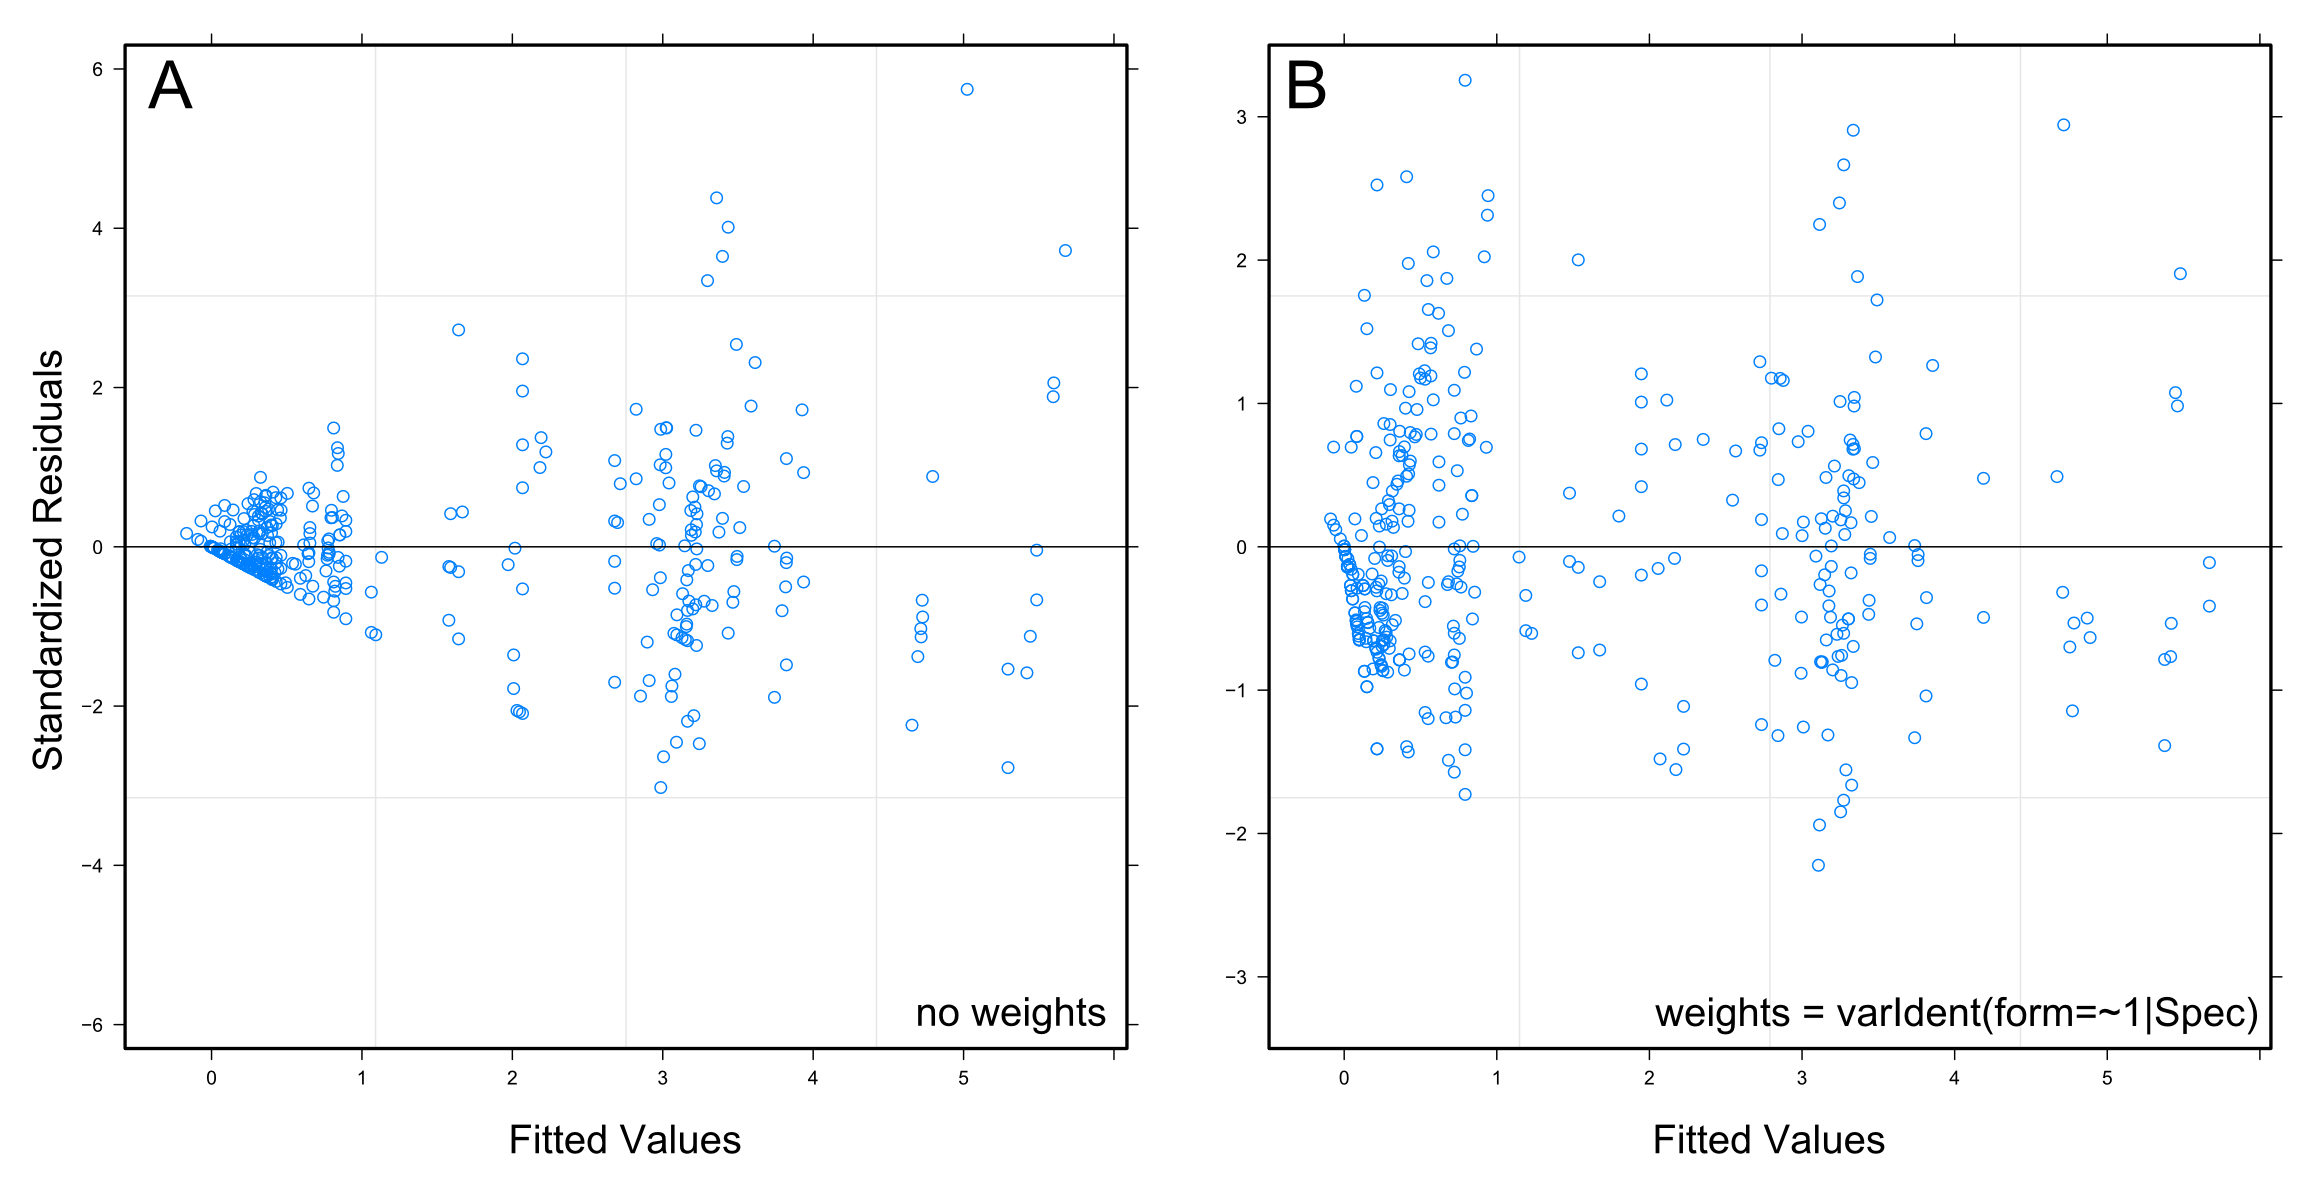
\includegraphics[width=15cm]{Images/residuals}
 \caption{Standardized residuals plotted against fitted values for the final mixed effect model with and without applied weighting. A) Without weighting, the residuals show strong pattern of heteroscedasticy. B) The weighting allows different variance per species. The final model is significantly better with weighting (\textit{L}=393.32, df= 4, \textit{P} $<$ 0.0001)}
 \label{fig:residuals}
\end{figure}

%%%%%%%%%%%%%%%%%%%%%%%%%%

\begin{table} [!htbp]
	\centering
	\caption{Extended output from the linear mixed effect model. Floral cover and species richness were removed in the model selection }
	\begin{tabular}{lccc}
		\toprule
		\textbf{Expanatory Variables} & \textbf{Estimate} & \textbf{$\pm$ SE} &  \textbf{\textit{P}} \\
		\midrule
		Intercept (Ger) & 1.41 & 0.49  & 0.0048 \\ 
		Lat	& -1.58 & 0.58 & 0.0069 \\ 
		Lot	& -1.38 & 0.51 & 0.0075 \\ 
		Ono	& -1.31 & 1.06 & 0.2182 \\ 
		TP	& -1.39 & 0.5  & 0.0060 \\ 
		\addlinespace[0.2cm]
		Frequency	& 0.11 & 0.05 & 0.0147 \\
		Frequency$^{2}$	& -0.002 &  $<$ 0.01 & 0.0699 \\ 
		Frequency$^{3}$	& $<$ 0.01 & $<$ 0.01 & 0.1174 \\ 
		\addlinespace[0.2cm]
		Frequency x Lat	& -0.09 & 0.05 & 0.0925 \\
		Frequency x Lot	& -0.09 &  0.05 & 0.0687 \\ 
		Frequency x Ono	& 0.32 & 0.14 & 0.0183 \\ 
		Frequency x TP	& -0.1 & 0.05 & 0.0425 \\
		\addlinespace[0.2cm] 
		Frequency$^{2}$ x Lat	& $<$ 0.01 & $<$ 0.01 & 0.1013 \\
		Frequency$^{2}$ x Lot	& $<$ 0.01 & $<$ 0.01 & 0.2053 \\ 
		Frequency$^{2}$ x Ono	& -0.01 & $<$ 0.01 & 0.0113 \\ 
		Frequency$^{2}$ x TP	& $<$ 0.01 & $<$ 0.01 & 0.1479 \\ 
		\addlinespace[0.2cm]
		Frequency$^{3}$ x Lat	& $>$ -0.01 & $<$ 0.01 & 0.0966 \\
		Frequency$^{3}$ x Lot	& $>$ -0.01 & $<$ 0.01 & 0.2996 \\ 
		Frequency$^{3}$ x Ono	& $<$ 0.01 & $<$ 0.01 & 0.0086 \\ 
		Frequency$^{3}$ x TP	& $>$ -0.01 & $<$ 0.01 & 0.2283 \\
		\bottomrule
	\end{tabular}
	\label{tab:summary} 
\end{table}

\newpage
%%%%%%%%%%%%%%%%%%%%%%%%%%%%%%%%%%%%%%%%%%%%%%%%%%%%%%%%%%%%%%%%%%%%%%%%


\begin{sidewaystable}[!htbp] %Parameter Values
	\footnotesize
	\centering
	\caption{The full set of parameters and default values used in the model. }
	\begin{tabular}{l l l l l l}
		\toprule
		\textbf{Parameter} & \textbf{Description} & \textbf{NetLogo-Type} & 		  \textbf{Type} & \textbf{Value} & \textbf{Reference} \\
		\midrule
		\addlinespace[0.2cm]
		\multicolumn{6}{l}{\textsc{Setup Parameters:}} \\ 
		\addlinespace[0.2cm]
		
		area  & "world" in NetLogo, defined by a grid of cells called patches &       & integer & 100x100 &  \\
		
		patch-size & Size of one grid-cell in NetLogo. Can be either a flower or grass &       & float & 0.1m² &  \\
		
		tick  & One time-unit in NetLogo &       & integer & 1s    &  \\
		
		flower-cover & Proportion of grid cells containing a flower & global & integer &       5, 10, 20, 30, 50 &  \\
		
		frequency & Proportion of flowers which are species A 	($Freq_{B} = 100 - Freq_{A}$)  & global & integer &   0-100\%    &  \\
		
		cluster-number & Average number of flowers per cluster & global & integer &  1, 2, 5, 10, 20, 50, 75, 100 &  \\
		
		number-bees & Initial number of pollinators in the model & global & integer &  10    & 0.0004 - 1 bee/m² \citep{essenberg2012explaining} \\
		
		\addlinespace[0.2cm]
		\multicolumn{ 6 } {l} {\textsc{Behavioural Parameters:}} \\ 
		
		search-speed & Distance a pollinator can move per tick & bees-own & integer & 0.1m /sec  & \begin{tabular}{@{}l@{}} \citealt{kunin1991few} in \citealt{kunin1996pollinator}  \\  0.09-0.17 \citep{essenberg2012explaining} \end{tabular} \\
		
		stdev-angle & Standard deviation for the normal distribution used in the CRW & global & integer &  30    & \citealt{waddington1980flight}  \\
		
		flightsteps-until-change & Seconds of unsuccessful search before the preference changes & bees-own & integer & 5s ( = 5 ticks) &  \citealt{chittka1997foraging,kunin1993sex}  \\
		
		length-memory & How many flowers can a bee remember to avoid double-visiting.  & bees-own & integer & 4     & \citealt{goulson2000pollinators}, see \citealt{goulson1999foraging} for review \\
		
		view  & Value for the radius of grid-cells a pollinator can see (cone-view of 180°) & bees-own & integer & 0.7m ( = 6 grid-cells) &  \begin{tabular}{@{}l@{}} \citealt{dyer2008comparative, wertlen2008detection} \\ \citealt{ne2001effect} \end{tabular} \\
		
		array & \begin{tabular}{@{}l@{}} Array of all suitable flowers (referred, non-visited)\\ in sight of the pollinator \end{tabular} & bees-own & Array &       &  \\
		
		reward-function & How much reward is regrowing per second & flowers-own & float & 0.00004 J/s   &  \\
		
		handling-time & The time a pollinator needs for exploiting the floral reward & bees-own & integer & reward * 4s + 0.5s (+ 3s) & \citealt{roubik1992ecology} in \citealt{kunin1996pollinator} \\
		
		reward & \begin{tabular}{@{}l@{}}Reward in Joule the flower has to offer. \\  Exploited with each visit, renewed over time \end{tabular} & flowers-own   & float & reward(max) = 1J & \citealt{kunin1991few} in \citealt{kunin1996pollinator}  \\
		
		pollen carry-over rate & Max. number of visits within a successful pollination is possible & flowers-own & integer & 1, 2, 4, 6, 8, 16  & \citealt{benadi2012population} \\
		
		flower-memory & A list of flower-locations  & bees-own & string &    4   & see \citealt{goulson1999foraging} for review) \\
		
		reward-memory & A list of the last gained rewards & bees-own & string &    4   &  \\
		
		change-prob & \begin{tabular}{@{}l@{}}Probability to change the preferred flower type. \\ Increases with low reward and long search times \end{tabular} & bees-own & float &       &  \\
		
		choice & Current flower choice for the pollinator (for constancy) & bees-own & boolean &       &  \\
		
		\bottomrule
	\end{tabular}%
	\label{tab:parametervalues}%
\end{sidewaystable}%


%%%%%%%%%%%%%%%%%%%%%%%%%%%%%%%%%%%%%%%%%%%%%%%%%%%%%%%%%%%%%%%%%%%%%%%%
\newpage


\begin{figure} [!h]
	\centering
	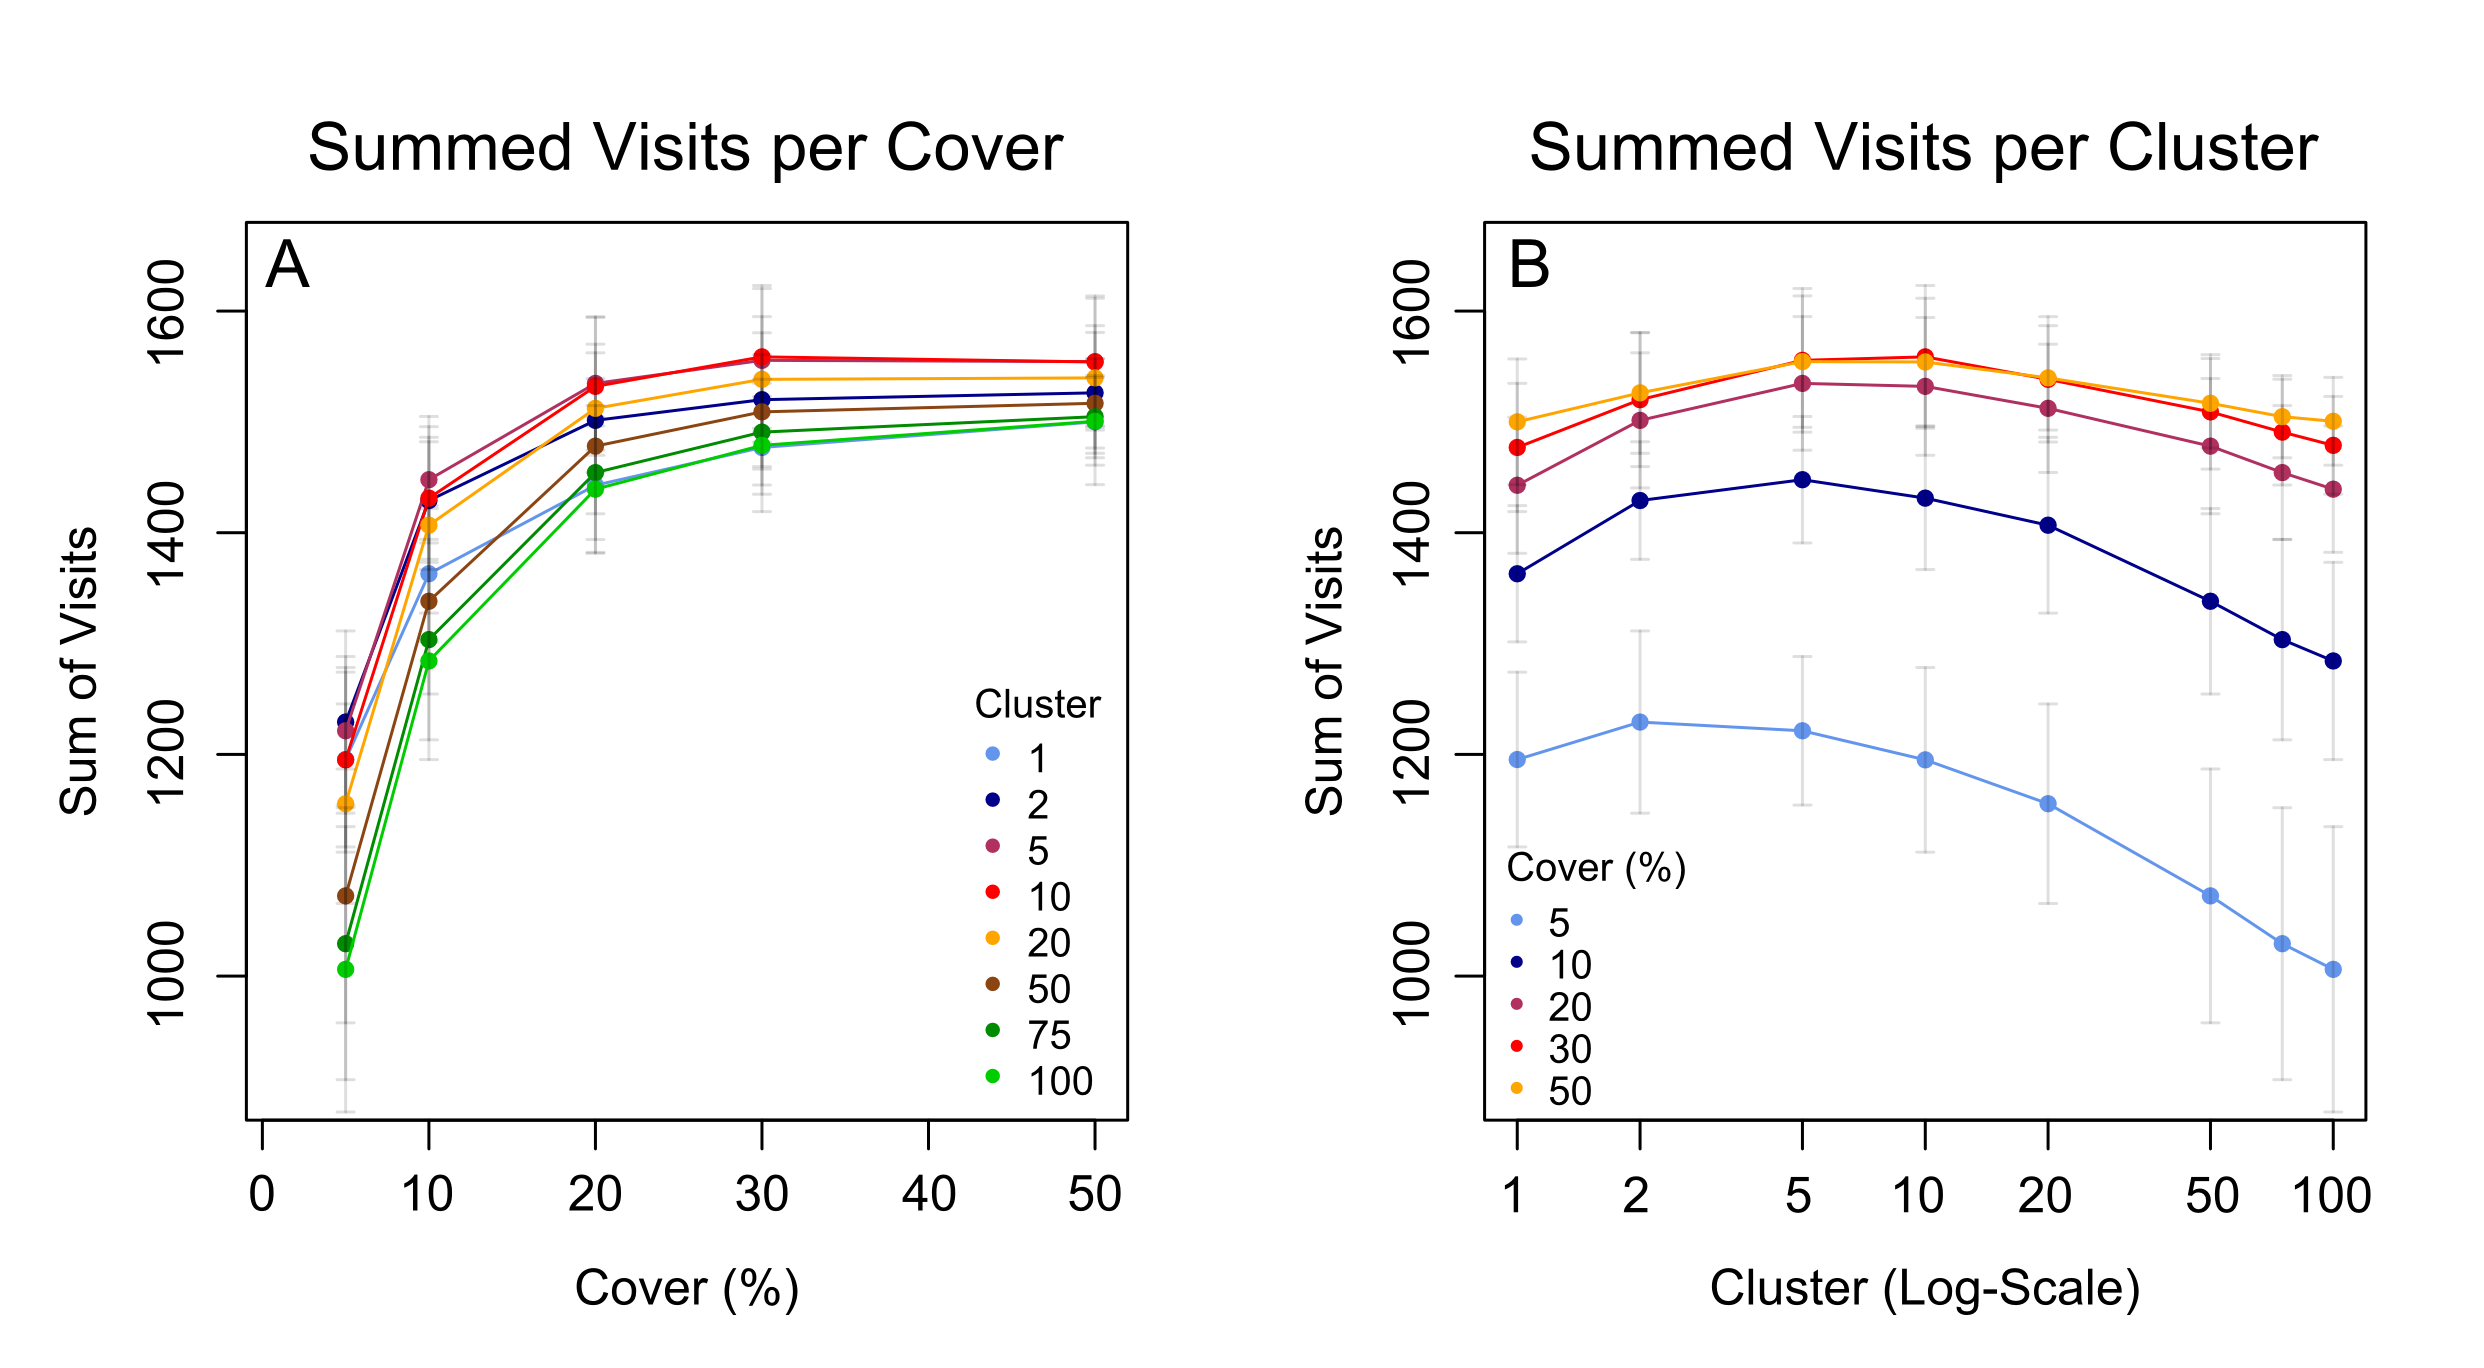
\includegraphics[width=14cm]{Images/nonfreq}
	\caption{Frequency independent influence of floral cover and degree of flower agglomeration on the summed visits within one simulation run. Cover strongly influences the number of visits as it reduces the flight and search time. Plot A shows a saturated relationship for all cluster values. This matches the Holling´s type II functional response. B) The degree of clustering also determines the sum of visits in a hump-shaped function. The maximum (depending on the cover) lays between 5 and 10 flowers per cluster. A small agglomeration of flowers reduces search times but keeps the next patch within short distance. The bigger the cluster, the more difficult to find the next one.}
	\label{fig:nonfreq}
\end{figure}

\clearpage

\begin{figure} [h!]
	\centering
	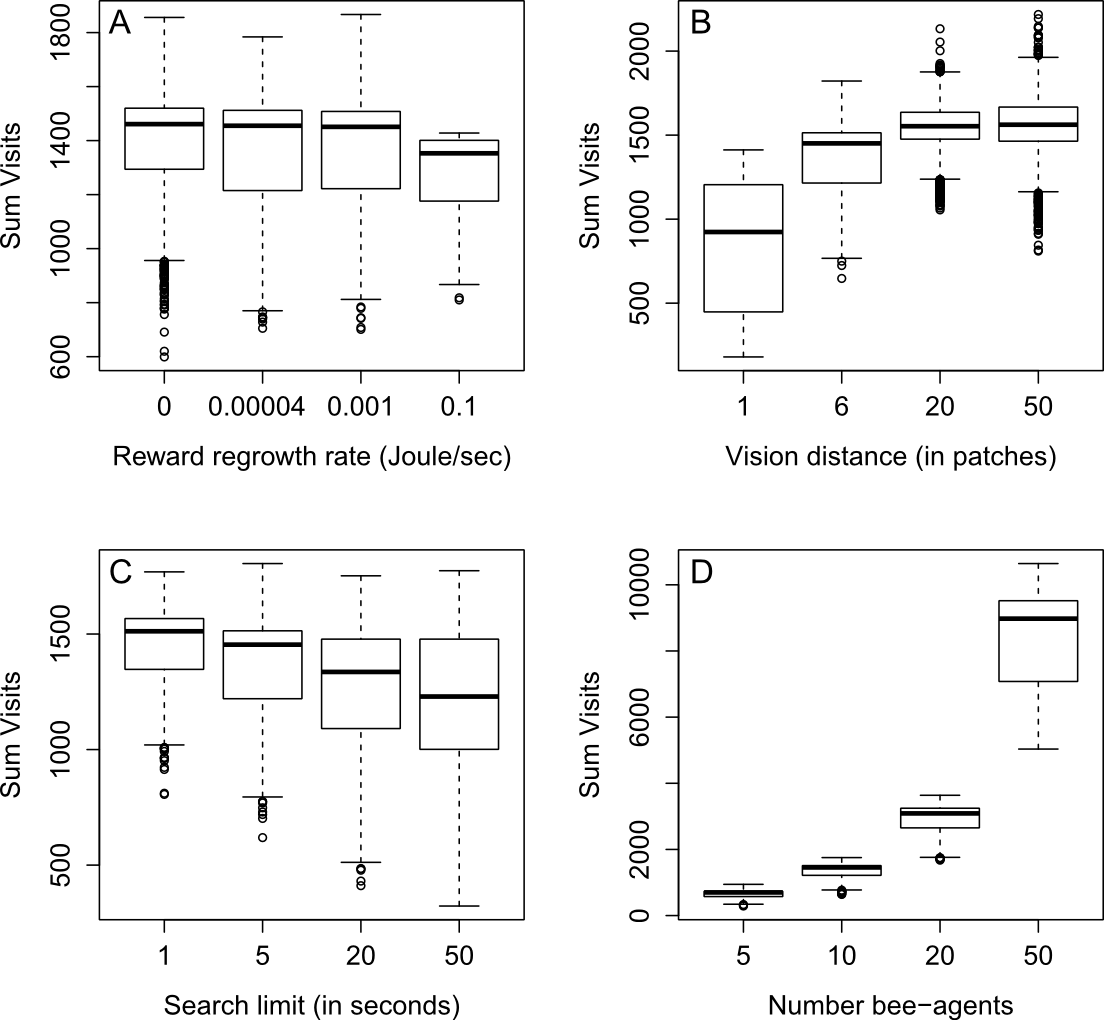
\includegraphics[width=14cm]{Images/SA_SUM}
	\caption{The influence of reward regrowth, vision, search limit and number of bee-agents on the total visits within a 1000 tick simulation run. A) Only an unnatural high reward regrowth has a small negative influence on the visits. B) Bee-agents with a far field of view can detect flowers faster, move in a direct way towards them and be therefore more efficient. However, the curve is saturated at a view of 20 patches. C) An increase in search time limit decreases the sum of visits and spread the variance. Bees-agents will keep searching for rare flowers instead of switching to the common species. D) As assumed, more bees lead to more visits.} 
	\label{fig:SA_SUM}
\end{figure}

\clearpage

\begin{figure} [!h] %
	\centering
	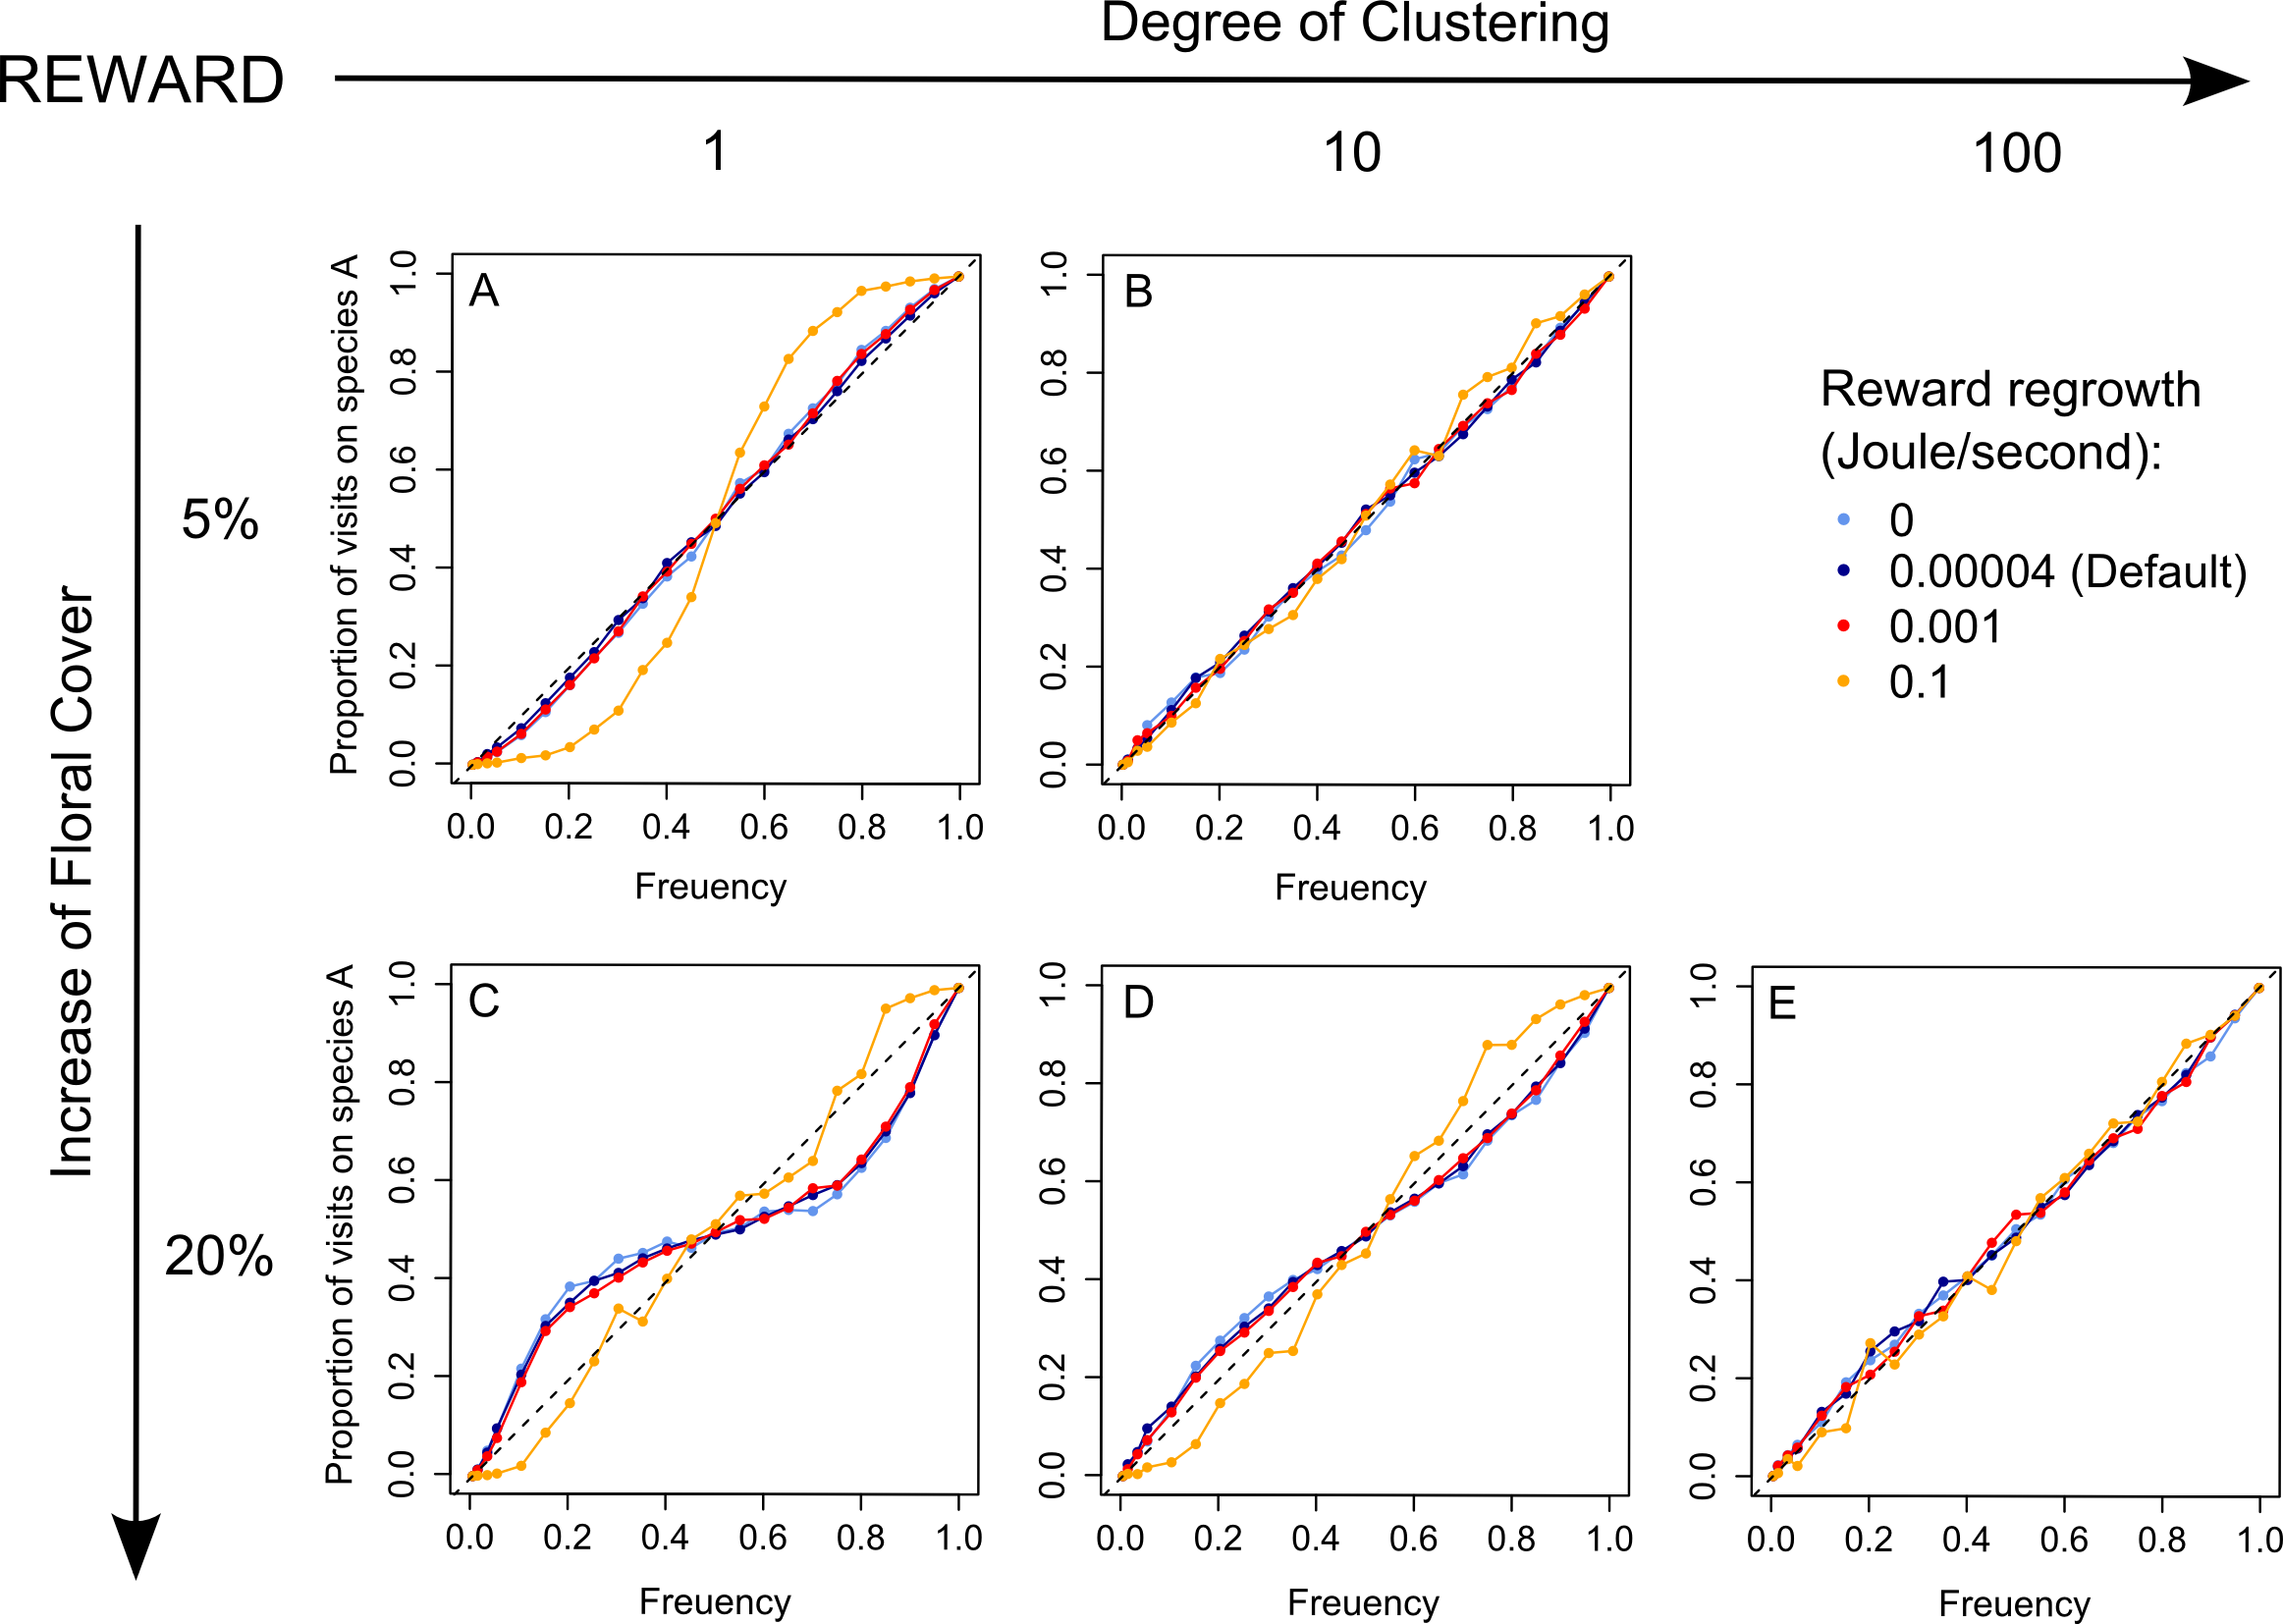
\includegraphics[width=14cm]{Images/SA_reward}
	\caption{Outcome of the model if the reward regrowth function is changed to 0, 0.004, 0.001 and 0.1 Joules per second. Only the unnatural high reward function (complete regrowth after 10 seconds) has an influence on the frequency dependence: the bee-agents have no more reason to change preference due to bad reward gained. This favors the more common species as shown in the opposite curving for no-cluster environments. A lower regrowth rate has no effect.} 
	\label{fig:SA_reward}
\end{figure}

\clearpage


\begin{figure} [!h]
	\centering
	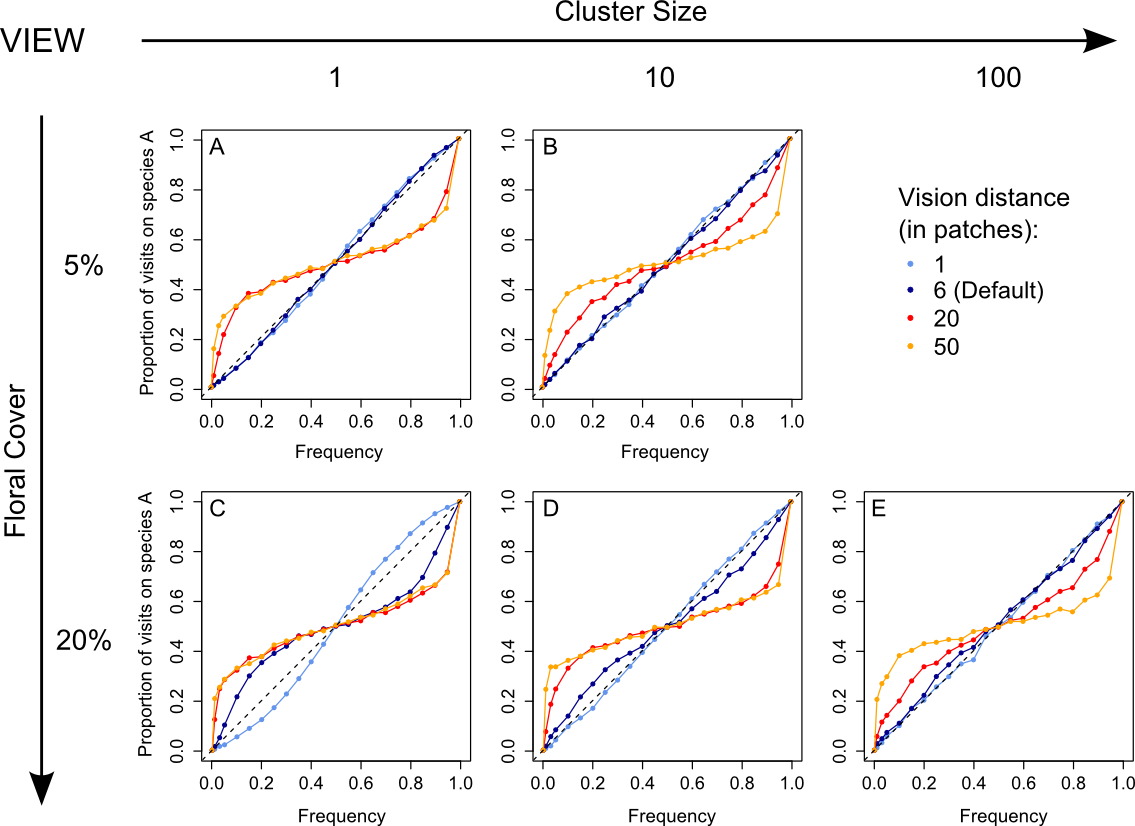
\includegraphics[width=14cm]{Images/SA_view}
	\caption{Effect of increased or reduced vision for the bee-agent. The vision influences the behavior of the bee-agent. If sees far, it can move on direct way towards the next preferred flower and saves searching time. But it also more often fly longer distances instead of changing to the common species. A high vision therefore increases the frequency dependence and a very low vision shifts the advantage towards the more abundant species.}
	\label{fig:SA_view}
\end{figure}

\clearpage


\begin{figure} [!h] 
	\centering
	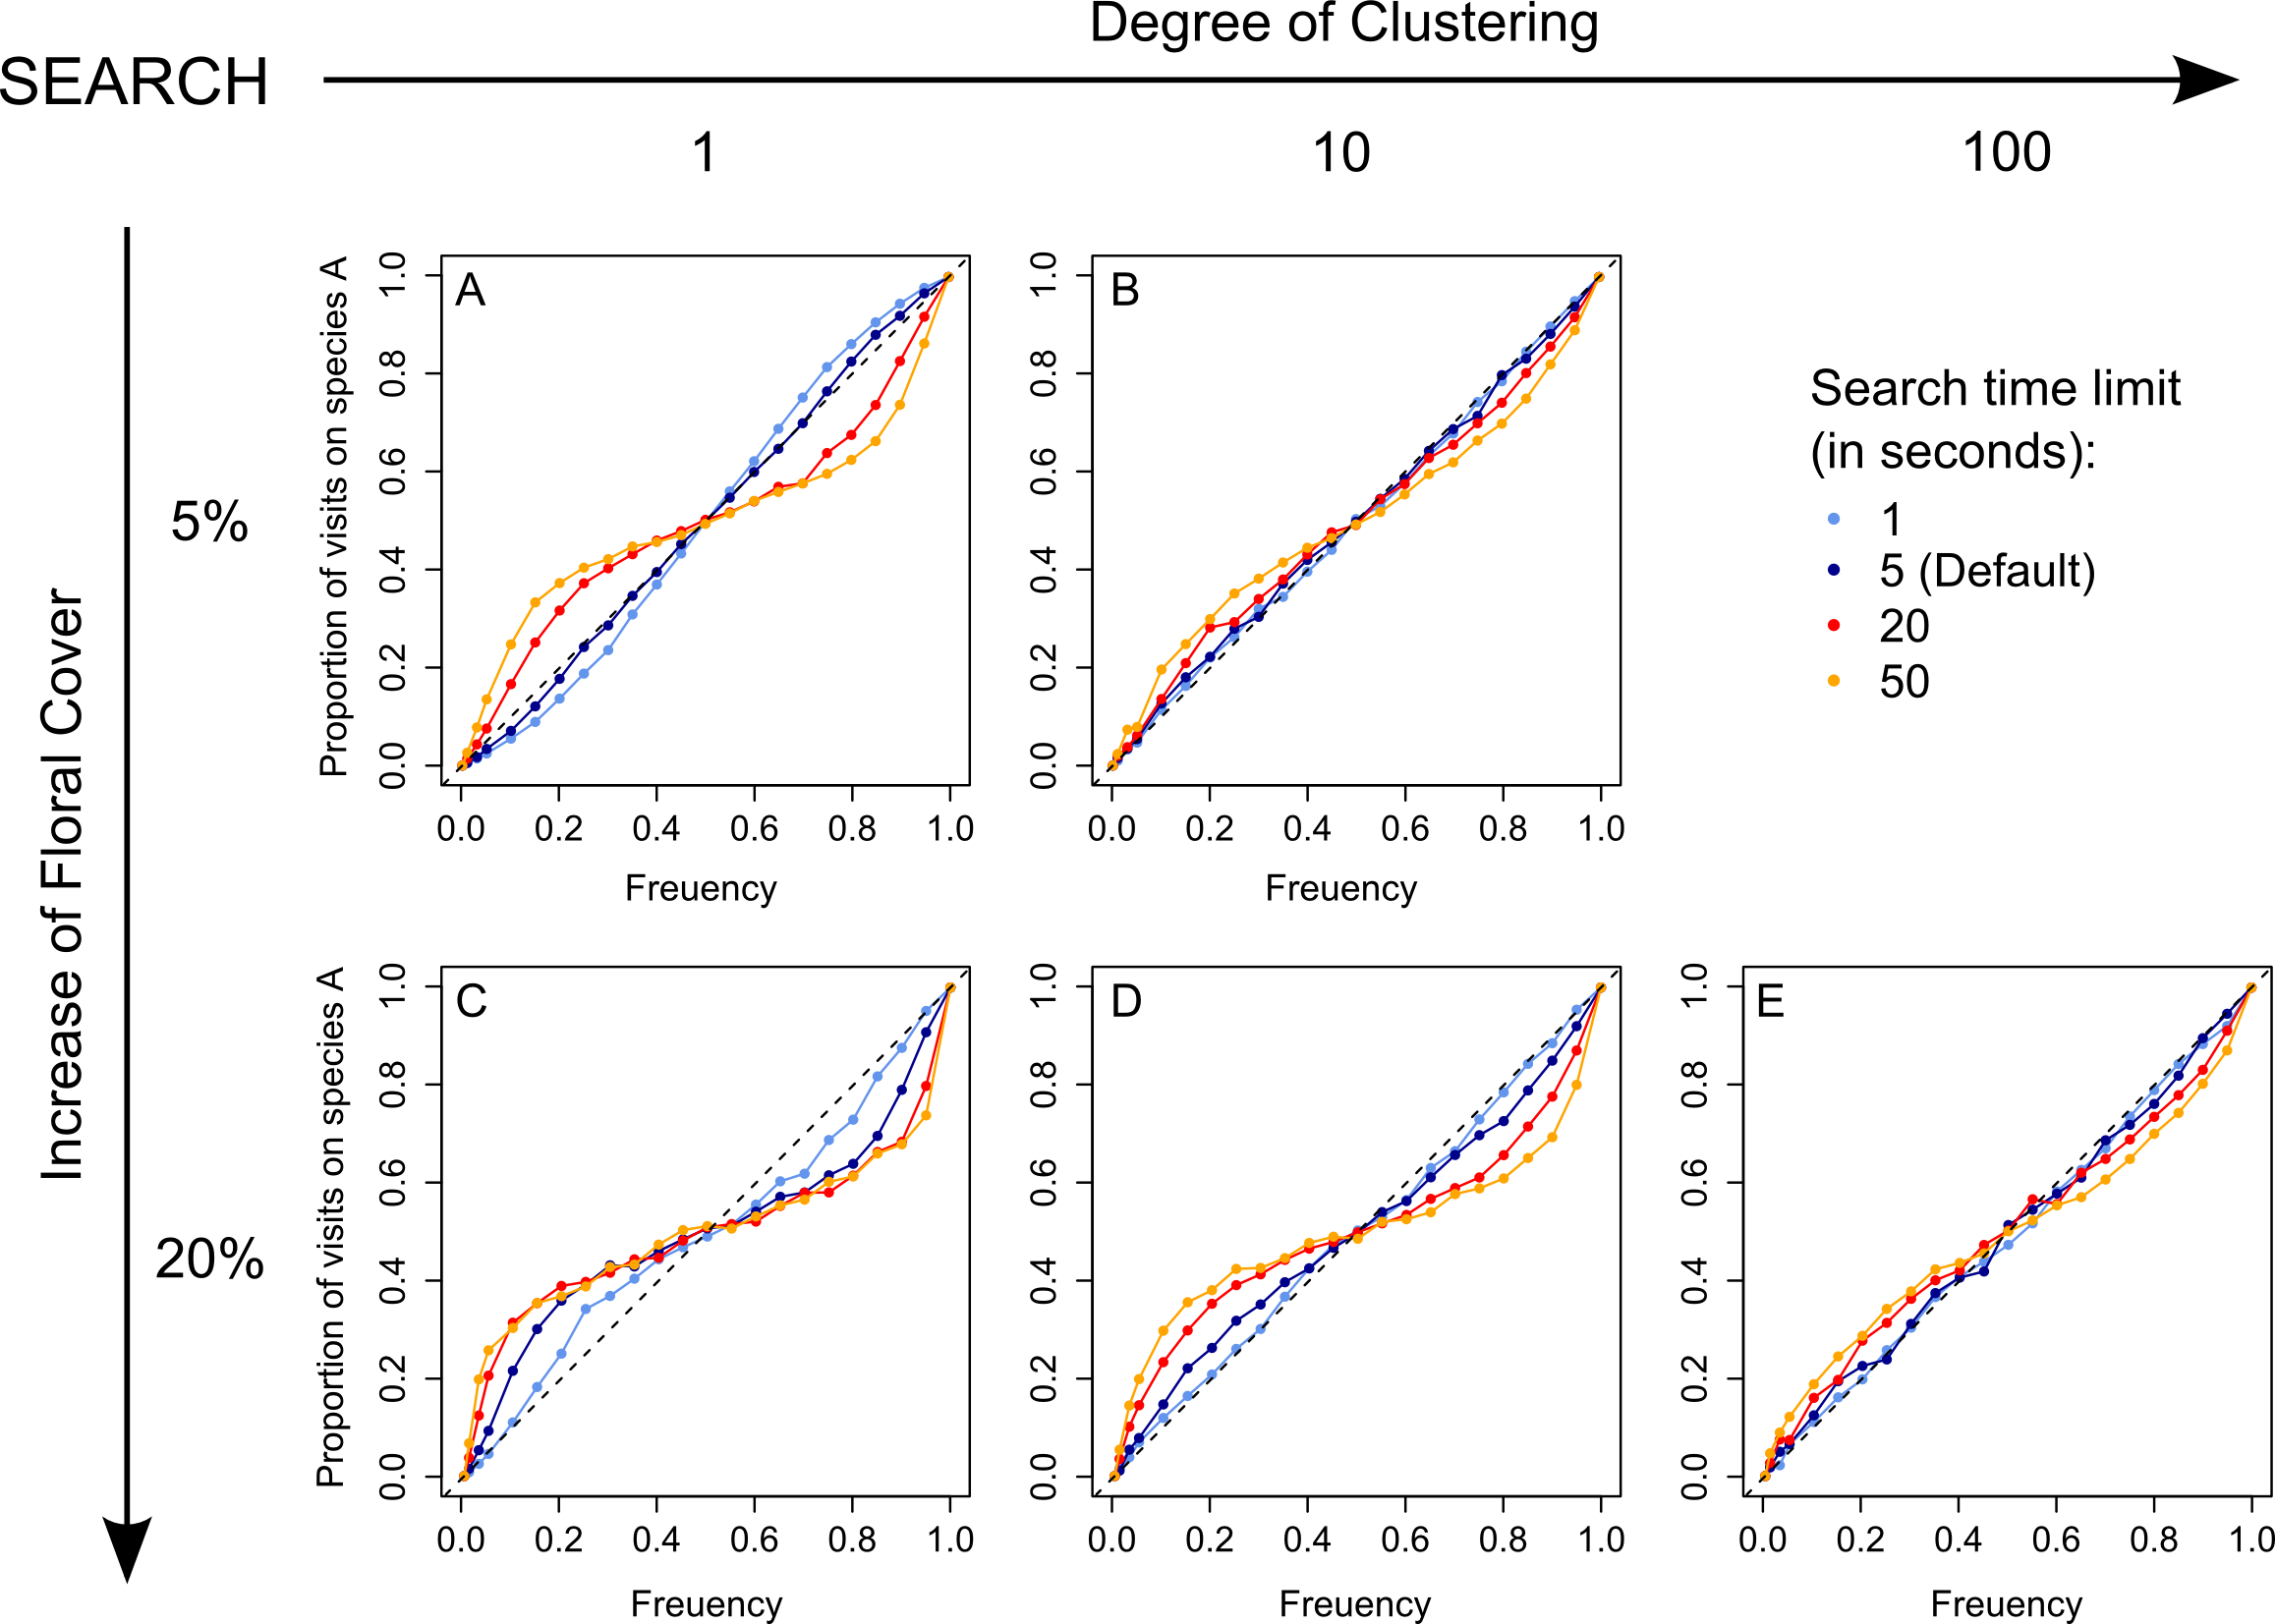
\includegraphics[width=14cm]{Images/SA_flight}
	\caption{Sensitivity analysis for search limits of 1,5, 20 and 50 seconds. The search limit is the number of seconds within a bee-agent searches for a unvisited and preferred flower, moving around the meadow by a correlated random walk. After the search limit is reached, the probability to change its flower preference increases with every additional second of unsuccessful search. The search limit has a similar effect on the outcome of the model as the vision because it also influences the change probability. With a higher search time, the bee-agent continues searing instead of switching to the more abundant flower, the frequency dependence is increased. A higher cluster value weakens the effect.}
	\label{fig:SA_flight}
\end{figure}

\clearpage

\begin{figure} [!h]
	\centering
	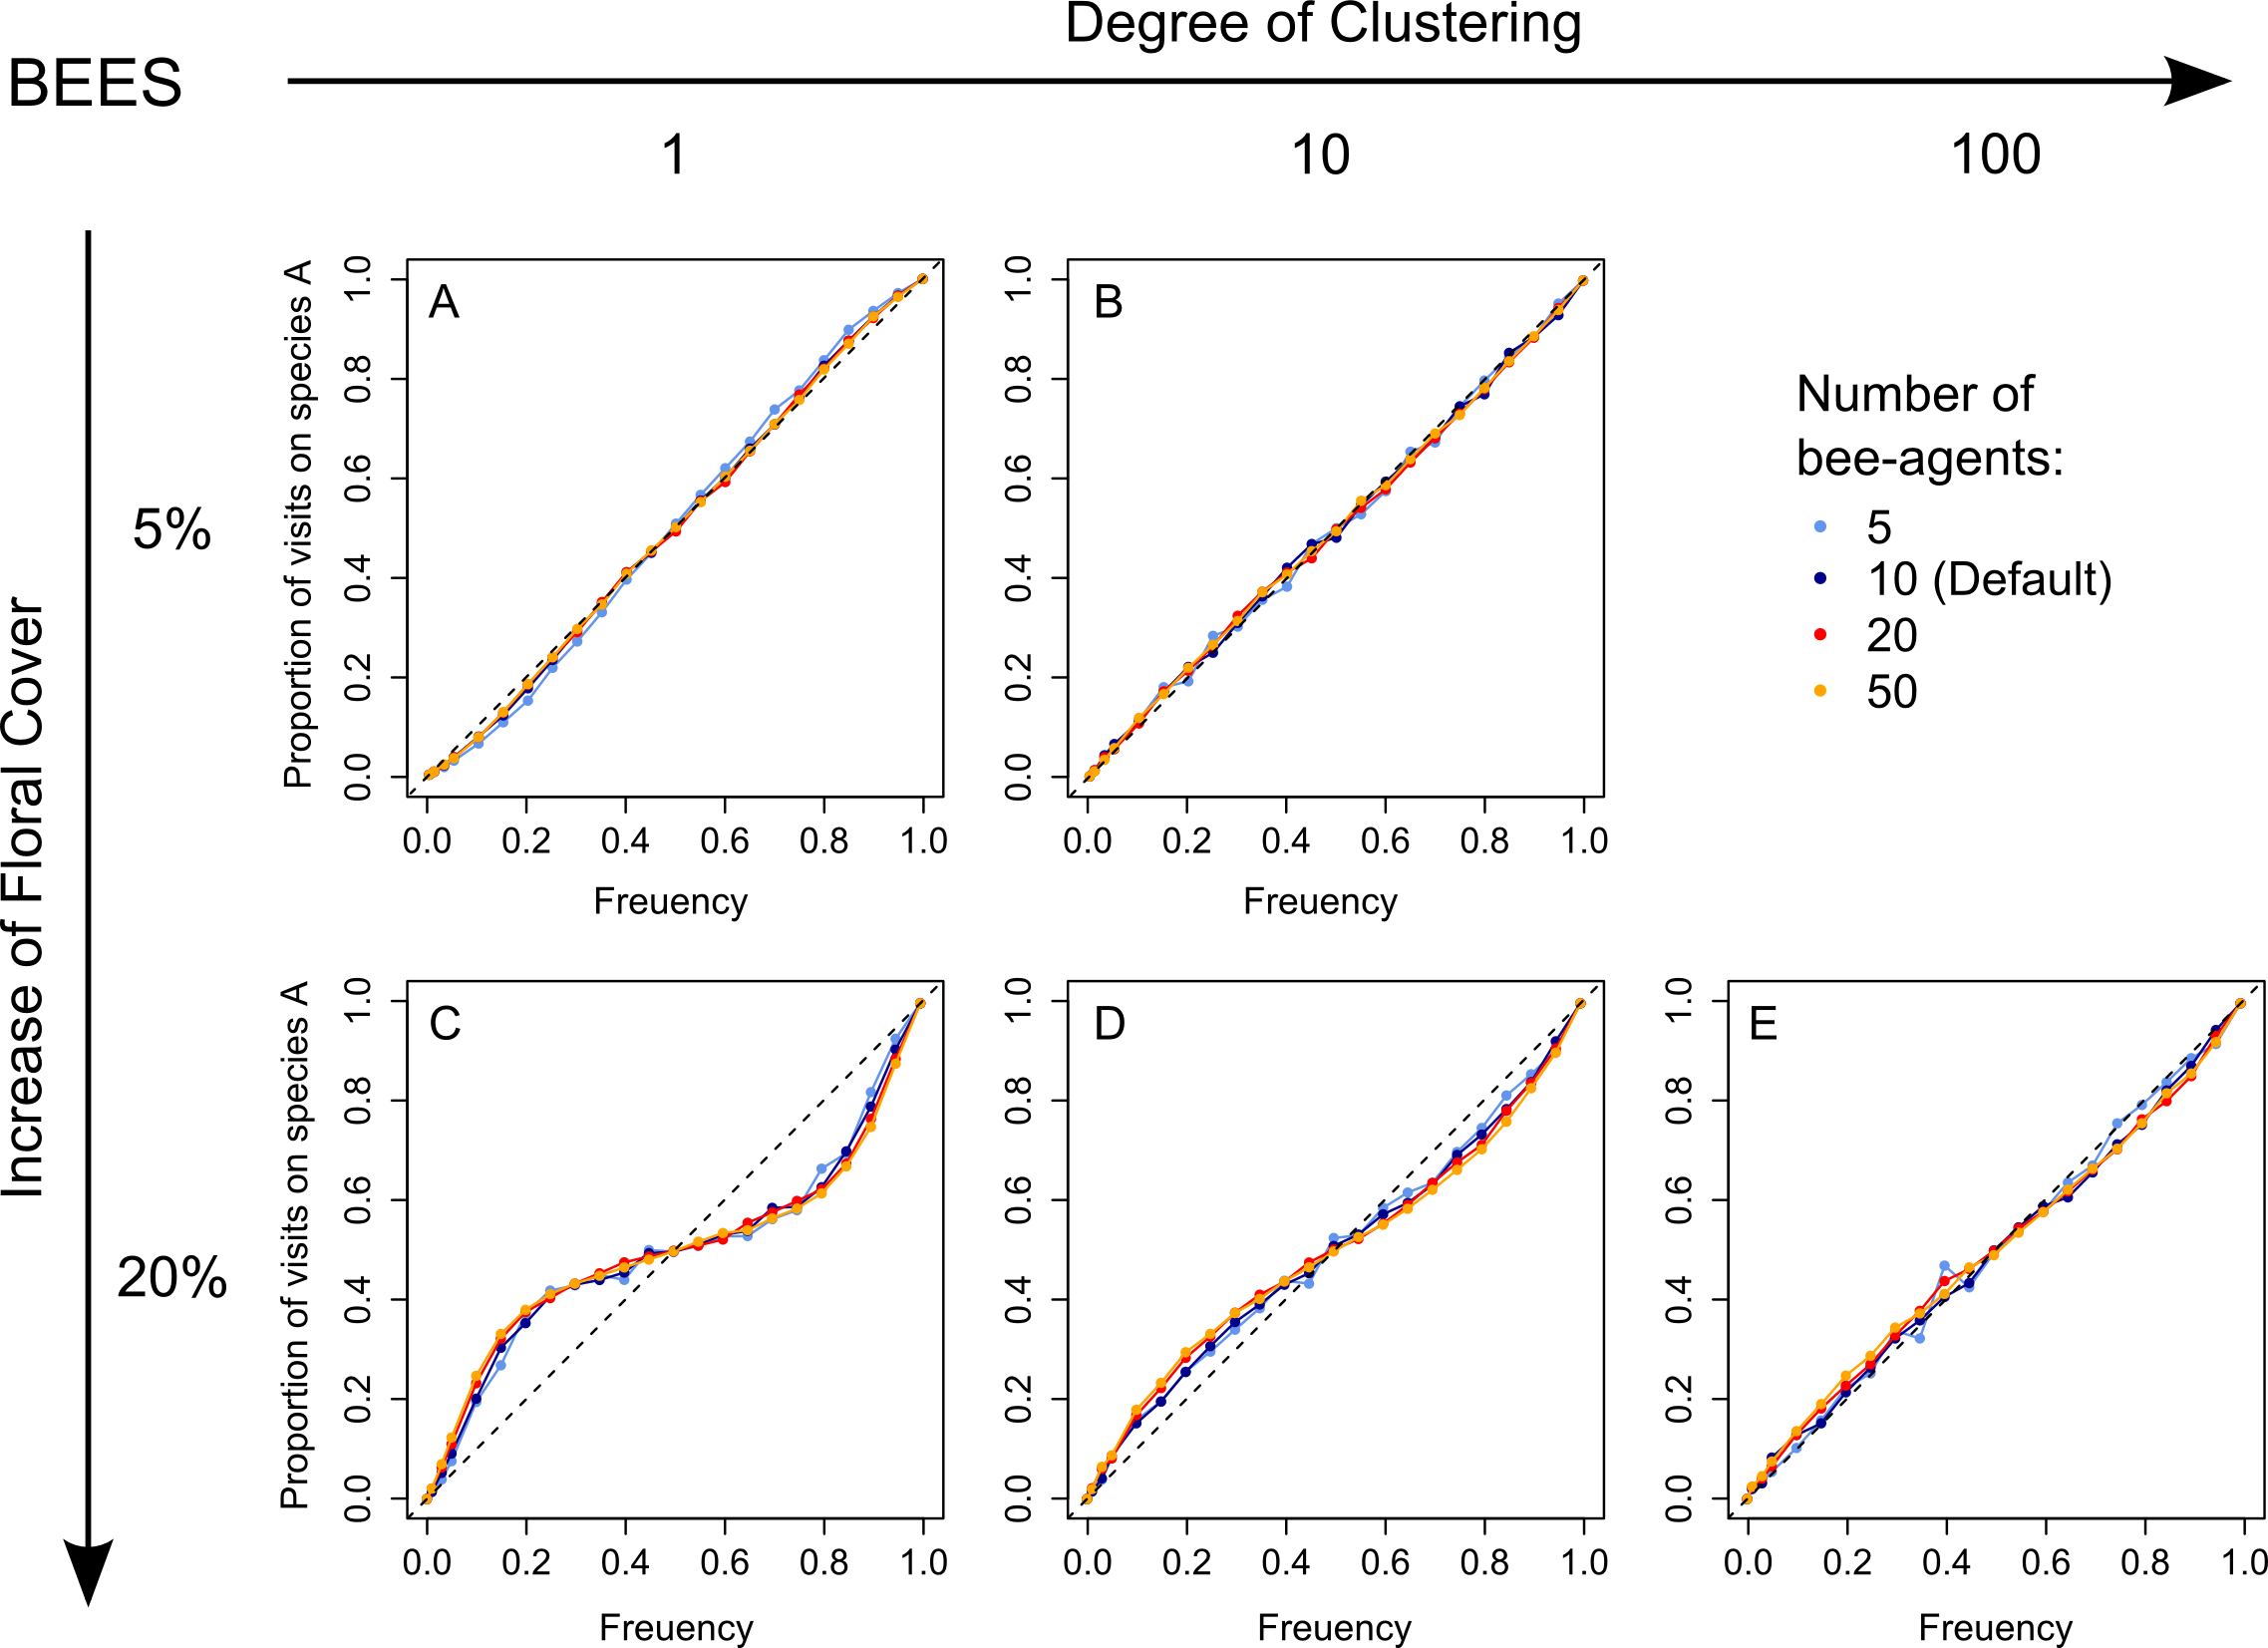
\includegraphics[width=14cm]{Images/SA_bees}
	\caption{Results of the model for 5, 10, 20 and 50 bee-agents on the meadow. The proportion of visits does not change, only the absolute numbers. Therefore has the pollinator density no influence on the frequency dependence.}
	\label{fig:SA_bees}
\end{figure}

%%%%%%%%%%%%%%%%%%%%%%%%%%%%%%%%%%%%%%%%%%%%%%%%%%%%%%%%%%%%%%%%%%%%%%%%

